\documentclass{article}
\usepackage[utf8]{inputenc}
\usepackage{pgfplots}
\pgfplotsset{width=6.6cm,compat=1.7}


\usepackage[backend=bibtex]{biblatex}
\addbibresource{sources.bib}

% has to be the last package to import
\usepackage{hyperref}
\hypersetup{
    colorlinks=true,
    citecolor=blue,
    linkcolor=black,
    filecolor=magenta,
    urlcolor=blue,
}
\urlstyle{same}

% Extra vertical spacing for each paragraph
\setlength{\parskip}{1em}


\title{Unity game performance difference between Vulkan and WebGL in Linux}
\author{Erik Reider}
\date{January 2021}


\begin{document}

% Title
\maketitle
\newpage

% Abstract
\begin{abstract}

\end{abstract}
\newpage


% Tabel of content
\tableofcontents
\newpage


\section {Introduction}
When creating a game, a programmer can choose where their game will be played. Depending on the platform, it could either be really simple or extremely difficult.The Unity game engine (also referred to as Unity) is a game creation tool that is considered to be one of the best game engines in the world. Unity can build games for Windows, Linux, Mac OS, Android, iOS, every modern console and your web browser.

\subsection {Background}
When compiling (building the project) towards Linux, the preferred graphics API (an acronym for Application Programming Interface) is Vulkan while the web browser uses WebGL2 (OpenGL ES 3.0 but will be referred to as WebGL). The graphics API makes it easier for the developers to render graphics more easily instead of writing code for every graphics card in existence\cite{APIWiki}. \par

OpenGL ES is a stripped down version of the regular more feature rich OpenGL while the differences between the latter and Vulkan is more stark. Vulkan is the successor to OpenGL which brings more asynchronous CPU optimizations and has less overhead but because of it being relatively new, it is not as widely adopted as OpenGL. Ergo, one of the reasons why WebGL uses OpenGL instead of Vulkan. One of the other reasons why WebGL doesn’t use Vulkan is because of the lack of native support for it on some platforms like Mac OS and iOS which uses OpenGL and Apple’s Metal API. Because of Vulkan being more efficient than OpenGL, it can process more draw calls in a given time than OpenGL. Draw calls are calls to the CPU that contains new materials, textures, objects, etc. Each call is then sent to the GPU for processing \cite{DrawCalls}. \par

Unity uses C\# (pronounced as "see sharp") is a Microsoft built programming language based off of the C languages. C\# was originaly intended to only be used on Microsofts Windows platform but then decided to sponsor an open-sourced implemntation of the language named Mono\cite{CSharpWiki}. Unity uses the Mono implemntation to be able to compile towards almost any platform.


\subsection {Description}
Because WebGL has a tendency of being less resource efficient than Vulkan, there should be an observable performance difference between the two, especially on lower end devices where the CPU performance isn’t the best. So focusing on CPU limited situations is an excellent way of benchmarking the differences. The benchmarks should be conducted on a low-end PC and a high-end PC to verify the performance differences. \par
To make the comparison as scientific as possible, the high-end PC’s CPU will be underclocked to 2.0GHz to simulate a lower-end PC with the same hardware to eliminate any differences except for the CPU. Those results will then be compared to the stock PC. While testing, the FPS will be logged.



\section {Material}
\subsection* {Unity 3D}
The game engine used to create and compile the benchmarks
\newline\href{https://unity.com}{Unity}

\subsection* {C\# and Mono}
The programming language and dotnet implemntation used.
\newline\href{https://www.mono-project.com/}{Mono}
\newline\href{https://docs.microsoft.com/en-us/dotnet/csharp/}{C\#}

\subsection* {NeoVim and Visual Studio Code}
The text editors used.
\newline\href{https://neovim.io/}{NeoVim}
\newline\href{https://code.visualstudio.com/}{Visual Studio Code}

\subsection* {Mozilla Firefox and Chromium}
The web browsers used to test WebGL
\newline\href{https://www.mozilla.org/en-US/firefox/new/}{Mozilla Firefox}
\newline\href{https://code.visualstudio.com/}{Chromium}


\subsection* {Github}
The reposetory host used to store all Unity files
\newline\href{https://github.com}{Github}

\subsection* {Courses}
The relevant courses are Programming 1, 2 and the digital creation course offered by \href{https://www.ntigymnasiet.se/}{NTI Gymnasiet}.


\section {Boundaries}
There will only be two benchmarks with 3 different APIs to test with three reruns to verify the performance results. Only two of the most popular browsers will be tested.

\section {TimeTable}
\begin{center}
\begin{tabular}{ |c|c| }
\hline
\textbf {Task} & \textbf {Time to spend} \\
\hline
Research CPU bound benchmarks & 1-2 days \\
\hline
Implement said benchmarks & 3 days \\
\hline
Run benchmarks, increase difficulty if needed & 1 day \\
\hline
Run benchmarks & 1 day \\
\hline
\end{tabular}
\end{center}


\section {Method}
The C\# code will generate each benchmark in realtime within the Unity engine. The first benchmark will generate a large 64x64 grid of cubes with random colors and Y position. On each tick (frame update), each cube will be destroyed and the grid gets created again with new materials. This should increase the amount of draw calls called. The second benchmark generates a ring of 256 cubes. On each tick, a new row gets generated with 2 more cubes than the last, building a cone. This benchmark also increases the amount of draw calls because of the sheer amount of cubes being added and visible at the same time.\par

Each hardware setup will run the benchmark three times to eliminate any anomalies while testing. All of the benchmarks will be ran with Vulkan, WebGL and with OpenGL as a control. To increase the reliability of the WebGL tests, both Firefox and Chromium (which Google Chrome is based off of) will be used to run the benchmark. Those browsers tend to be the most popular choices\cite{WebBrowsers}. While running the benchmark, the FPS will be logged and averaged into separate files per run to ease the comparison between different results and to eliminate any inevitable mistakes. The first benchmark will run for 30 seconds meanwhile the second benchmark will run until the fps (acronym for frames per second) drops below 10. Before running the benchmarks, all non essential programs like Discord, Spotify, Steam will be killed to further eliminate any strange deviations between each run. To make the benchmark more CPU bound, all settings will be set to the lowest value which will increase the performance delta if there is one.

\subsection {PC specifications}
\begin{itemize}
    \item CPU: AMD Ryzen 7 5800X
    \item CPU performance profile: Performance
    \item Graphics driver: Mesa 21.1.0-devel (git-e2608312d3)
    \item Resolution: 1920x1080
    \item OS and kernel: Linux 5.10.14-119-tkg-upds
\end{itemize}


\section {Results and analysis}
Figure[\ref{fig:test1}] shows a massive difference between both platforms while on each platform, the differences are very minutiae. This graph shows the averaged fps which means that a higher number is always better but, within around a 8\% range the differences do not matter. OpenGL is around 3fps faster than Vulkan while both browsers perform the same. The performance drop from stock CPU clock speeds to 2GHz is enormous at a 50\% drop in performance. The high-end PCs native performance is around 6.75 times faster than both web browsers. The difference on the low-end PC was exponentially larger at an eye-watering 1000\% performace increase.

The results from figure[\ref{fig:test2}] are not as drastically different from each other compared to figure[\ref{fig:test1}] but there is still a difference. This test measures time instead of fps meaning that a larger number results in a higher and a more stable fps. Vulkan lasted for 3 seconds longer than OpenGL on both systems while lasting 7.5 averaged seconds longer than the web results. The OpenGL results on both systems lasted an averaged 3.75 seconds longer than both web browsers.

\section {Discussion}
Using the data collected, The performance difference between WebGL and Vulkan is ginormous, especially on lower-end hardware where performance really matters. 

\section {Conclusion}




% References
\printbibliography[heading=bibnumbered,title={References}]

% Figures
\newpage\section {Figures}

\begin{figure}[!ht]
\center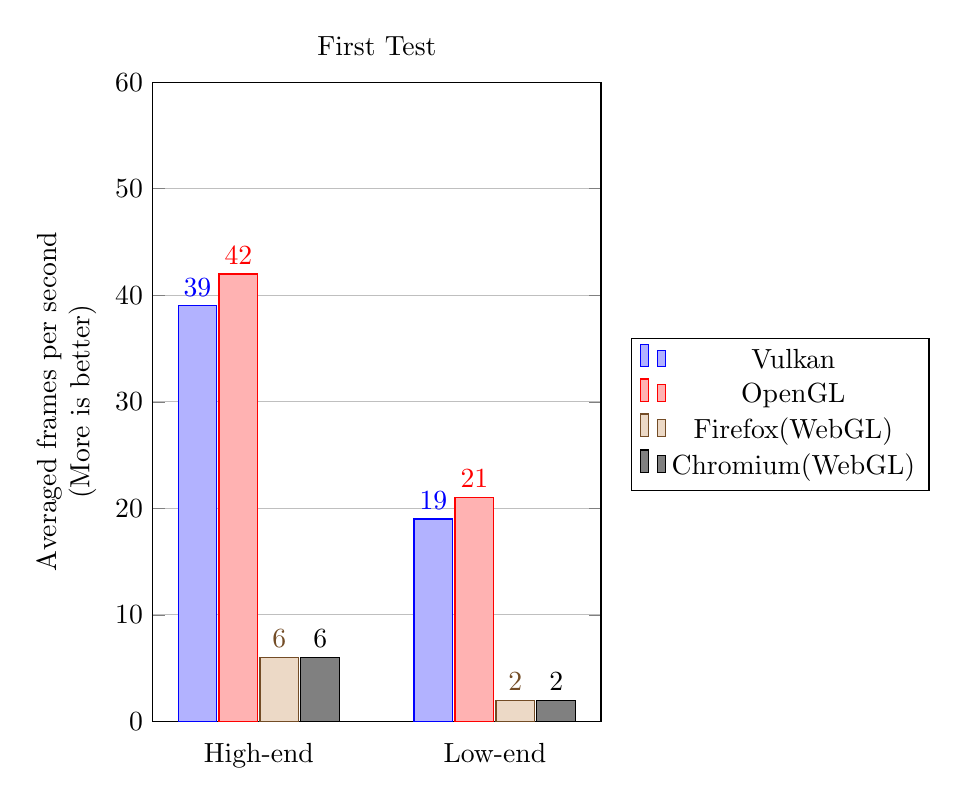
\begin{tikzpicture}
\begin{axis} [
    title = First Test,
    ylabel style={align=center}, ylabel=Averaged frames per second\\(More is better),
    nodes near coords,
    nodes near coords align={vertical},
    width = 0.6*\textwidth,
    height = 0.8*\textwidth,
    major x tick style = transparent,
    ybar=2*\pgflinewidth,
    bar width=14pt,
    ymajorgrids = true,
    symbolic x coords={High-end, Low-end},
    xtick = data,
    scaled y ticks = false,
    enlarge x limits=0.45,
    ymin=0,
    ymax=60,
    legend style={at={(1.4, 0.6)}, anchor=north},
]
\addplot coordinates {(High-end, 39) (Low-end, 19)}; %Vulkan
\addplot coordinates {(High-end, 42) (Low-end, 21)}; %OpenGL
\addplot coordinates {(High-end, 6) (Low-end, 2)}; %Firefox
\addplot coordinates {(High-end, 6) (Low-end, 2)}; %Chromium
\legend{Vulkan, OpenGL, Firefox(WebGL), Chromium(WebGL)}
\end{axis}
\end{tikzpicture}
\caption{Colored Cubes Test}
\label{fig:test1}
\end{figure}

\begin{figure}[!ht]
\center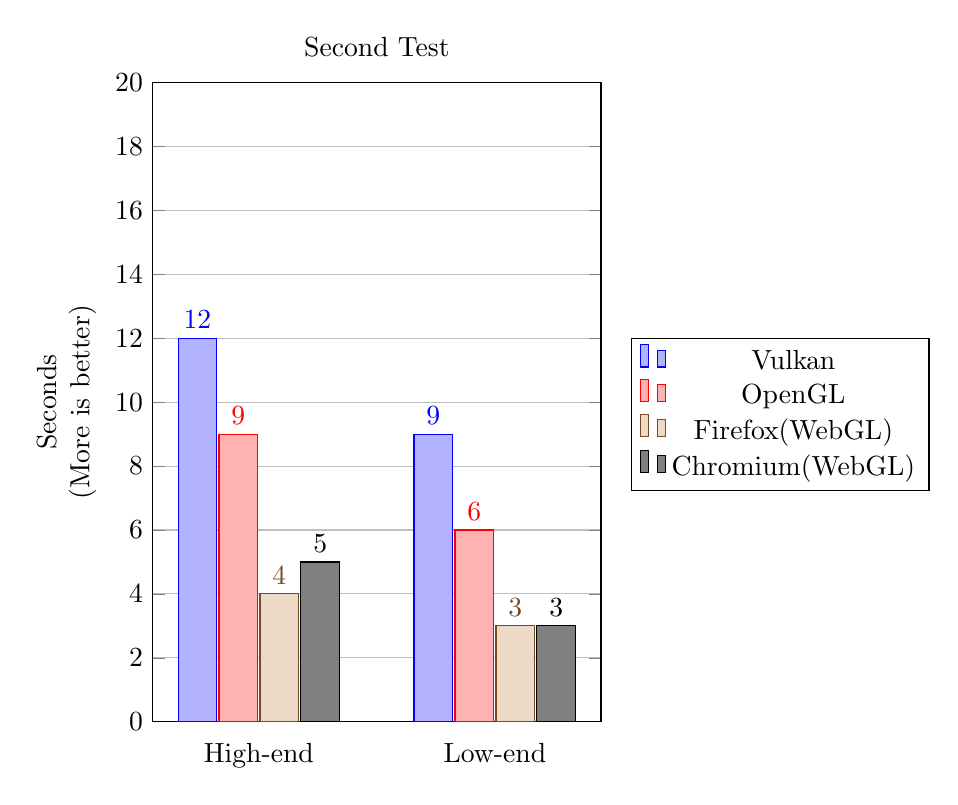
\begin{tikzpicture}
\begin{axis} [
    title = Second Test,
    ylabel style={align=center}, ylabel=Seconds\\(More is better),
    nodes near coords,
    nodes near coords align={vertical},
    width = 0.6*\textwidth,
    height = 0.8*\textwidth,
    major x tick style = transparent,
    ybar=2*\pgflinewidth,
    bar width=14pt,
    ymajorgrids = true,
    symbolic x coords={High-end, Low-end},
    xtick = data,
    scaled y ticks = false,
    enlarge x limits=0.45,
    ymin=0,
    ymax=20,
    legend style={at={(1.4, 0.6)}, anchor=north},
]
\addplot coordinates {(High-end, 12) (Low-end, 9)}; %Vulkan
\addplot coordinates {(High-end, 9) (Low-end, 6)}; %OpenGL
\addplot coordinates {(High-end, 4) (Low-end, 3)}; %Firefox
\addplot coordinates {(High-end, 5) (Low-end, 3)}; %Chromium
\legend{Vulkan, OpenGL, Firefox(WebGL), Chromium(WebGL)}
\end{axis}
\end{tikzpicture}
\caption{Colored Cone test}
\label{fig:test2}
\end{figure}



\end{document}
